\chapter{Background\label{chap:background}}

\section{The Linux scheduler\label{sec:LinuxSched}}

The process scheduler is the component of the kernel that selects
which process to run next. Processor time is a finite resource, and the
process scheduler (or simply the \emph{scheduler}) is a subsystem of
the kernel that assigns processor time to the runnable processes.

In a single processor machine, the scheduler gives the impression
to the user that multiple processes are executing simultaneously.
This is the basis of a \emph{multitasking}\footnote{In this context \emph{task}
and \emph{process} are used as synonyms.} operating system like Linux.

On multiprocessor machines processes can actually run concurrently (in
parallel) on different processors. The scheduler has to assign runnable
processes to processors and decide, on each of them, which process to run. 

How the scheduler works affects how the system behaves. We can privilege task
switching in order to have a reactive and interactive system, we can allow
tasks to run longer and have a batch jobs well suited system, we can also
decide that some tasks are vital for the system and must execute to the
detriment of the others.

\subsection{Modular scheduling framework\label{sec:LinuxSched_structure}}

The current version of the Linux scheduler has been designed and implemented by Ingo
Molnar~\cite{molnar07} as a modular framework that can easily be extended.
Each scheduler module is a \emph{scheduling class} that encapsulate specific
scheduling policies details.

Scheduling classes are implemented through the \texttt{sched\_class}\footnote{
Defined in \texttt{include/linux/sched.h}.} structure, which contains hooks to
functions that must be called whenever the respective event occurs. A (partial)
list of scheduler hooks is:
\begin{itemize}
\item \texttt{enqueue\_task(...)}: it is called when a task enters a runnable state.
It enqueues a task in the data structure used to keep all runnable tasks
(runqueue, see below).
\item \texttt{dequeue\_task(...)}: it is called when a task is no longer runnable. It
removes a task from the runqueue.
\item \texttt{yield\_task(...)}: it yields the processor giving room to the
other tasks to be run.
\item \texttt{check\_preempt\_curr(...)}: it checks if a task that entered the
runnable state should preempt the currently running task.
\item \texttt{pick\_next\_task(...)}: it chooses the most appropriate task
eligible to run next.
\item \texttt{put\_prev\_task(...)}: it preempts a running task.
\item \texttt{select\_task\_rq(...)}: it chooses on which runqueue (CPU) a
waking-up task has to be enqueued.
\item \texttt{task\_tick(...)}: mostly called from the time tick functions,
it executes periodical stuff related  to the running task.
\end{itemize}
Three \emph{``fair''} scheduling policies
(\texttt{SCHED\_NORMAL}, \texttt{SCHED\_BATCH}, \texttt{SCHED\_IDLE}) and two
\emph{real-time} scheduling policies (\texttt{SCHED\_RR}, \texttt{SCHED\_FIFO}) are currently implemented in the Linux scheduler.
The situation is depicted in \figurename~\vref{fig:modular_scheduler}.

\begin{figure}[htbp]
    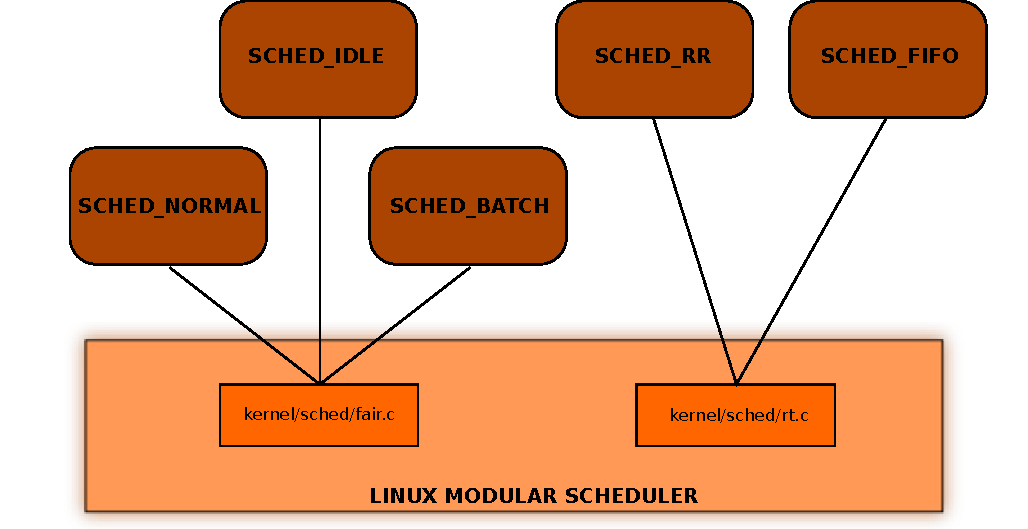
\includegraphics[width=\columnwidth]{images/modular_scheduler}
    \caption{The Linux modular scheduling framework.}
    \label{fig:modular_scheduler}
\end{figure}

\subsection{Scheduling entities, tasks and runqueues\label{sec:LinuxSched_runqueue}}
All data used by the scheduler to implement any scheduling policy are
contained into \texttt{struct sched\_entity}\footnote{Defined in
  \texttt{include/linux/sched.h}.} (there is a \emph{scheduling
  entity} for each scheduler module). Looking inside that structure we
find the fields (e.g.  \texttt{exec\_start}, \texttt{vruntime},
etc\dots) that the CFS\footnote{\emph{Completely Fair Scheduler}, the
  default Linux scheduler, see~\cite{sched-design-CFS}.} scheduler
uses to carry out his job.  The concept of \emph{scheduling entity} is
essentially ``something to be scheduled'', which might not be a
process (e.g. tasks groups~\cite{corbet07}).

At the very beginning of the \texttt{struct task\_struct}\footnote{Defined in
\texttt{include/linux/sched.h}.}
there are the fields that identify the tasks. Among others:
\begin{itemize}
\item \texttt{volatile long state}: it describes the task's state. It can assume
three values (\texttt{-1}, \texttt{0}, \texttt{>0}) depending on the task
respectively beeing \emph{unrunnable}, \emph{runnable} or \emph{stopped}.
\item \texttt{const struct sched\_class *sched\_class}: it binds the task to
his scheduling class.
\item \texttt{struct sched\_entity se}, \texttt{struct sched\_rt\_entity rt}: it 
contains \emph{scheduling entity} related informations.
\item \texttt{cpumask\_t cpus\_allowed}: mask of the cpus on which the task can
run.
\item \texttt{pid\_t pid}: process identifier that uniquely identifies the
task.
\end{itemize} 

Last but not least, we have runqueues. Linux has a main per-CPU runqueue data
structure called (not surprisingly) \texttt{struct rq}\footnote{Defined in
\texttt{kernel/sched.h}, with all runqueue related things.}. Runqueues are
implemented in a modular fashion as
well. The main data structure contains a ``sub-runqueue'' field for each
scheduling class, and every scheduling class can implement his runqueue in
a different way.

To better understand the inner working of the scheduler, it is
enlightening to look at the CFS runqueue implementation. Structure
\texttt{struct cfs\_rq} holds both accounting informations about
enqueued tasks and the actual runqueue. CFS uses a time-ordered
red-black tree to enqueue tasks and to build a ``timeline'' of future
task execution.

A red-black tree is a type of self-balancing binary search tree. For
every running process there is a node in the red-black tree. The
process at the left-most position is the one to be scheduled next. The
red-black tree is complex, but it has a good worst-case running time
for its operations and is efficient in pratice: it can search, insert
and delete in $O(\log n)$ time, where $n$ is the number of elements in
the tree. The leaf nodes are not relevant and do not contain data. To
save memory, sometimes a single sentinel node performs the role of all
leaf nodes.

Scheduling class designers must cleverly choose a runqueue
implementation that best fits scheduling policies
needs. \figurename~\vref{fig:runqueues} presents the structure of the
run-queues.

\begin{figure}[htbp]
    \includegraphics[width=\columnwidth]{images/runqueues}
    \caption{The CFS runqueue.}
    \label{fig:runqueues}
\end{figure}

\section{The Linux real-time scheduler}

Linux has been designed to be a general-purpose operating system
(GPOS), therefore it presents some issues, like unpredictable
latencies, limited support for real-time scheduling, and coarse-grain
timing resolution that might be a problem for real-time
application~\cite{LipariScordino2006}. The main design goal of the
Linux kernel has been (and still remains) to optimise the average
throughput (i.e., the amount of ``useful work'' done by the system in
the unit of time).

Since Linux is a POSIX-compliant operating system, the Linux scheduler
must also provide \texttt{SCHED\_FIFO} and \texttt{SCHED\_RR}
scheduling algorithms. These algorithms are actually implemented
inside the \texttt{SCHED\_RT} scheduling class, and so they represent
the part of Linux kernel code dedicated to real-time tasks
management. In this section we provide a brief explanation of those
classes, with an inspection to the implementation code, with
particular reference to multiprocessor systems support.

\subsection{SCHED\_FIFO and SCHED\_RR}\label{sec:StateArt_FIFO}

\texttt{SCHED\_FIFO} and \texttt{SCHED\_RR} are simple fixed-priority
policies. According to the POSIX standard\footnote{IEEE Std
  1003.1b-1993}, \texttt{SCHED\_FIFO} is a strictly first in-first out
(FIFO) scheduling policy.  This policy contains a range of at least 32
priorities (actually, 100 inside Linux). Tasks scheduled under this
policy are chosen from a thread list ordered according to the time its
tasks have been in the list without being executed. The head of the
list is the task that has been in the list the longest time; the tail
is the task that has been in the list the shortest
time.

\texttt{SCHED\_RR} is a round-robin scheduling policy with a
per-system time slice, named \emph{time quantum}. This policy contains
a range of at least 32 priorities and is identical to the
\texttt{SCHED\_FIFO} policy with an additional rule: when the
implementation detects that a running process has been executed for an
interval equal or greater than the time quantum, the task becomes the
tail of its task list, and the head of that task list is removed and
made a running task.

Both \texttt{SCHED\_FIFO} and \texttt{SCHED\_RR} unfortunately
diverges from what the real-time research community refer to as
``realtime''~\cite{buttazzo06}. 
Notable drawbacks of fixed priority schedulers are the fairness
and the security among processes~\cite{abeni06}. In fact, if a regular
non-privileged user is enabled to access the real-time scheduling
facilities, then he can also rise his processes to the highest
priority, starving the rest of the system.

\subsection{Multiprocessor support\label{sec:LinuxSched_multiproc}}

Since now, we have not addressed the issue of how many processor our
system has. In fact all that we have said remains the same for
uni-processor and multi-processor machines as well.

A multiprocessor Linux kernel (that is, one configured with \texttt{CONFIG\_SMP} flag set,
see Section~\ref{sec:SMP_UP} for more details) has additional fields into the afore-mentioned 
structures in comparison to a uniprocessor one.

In \texttt{struct sched\_class} we find:
\begin{itemize}
\item \texttt{select\_task\_rq(\dots)}: it is called from \texttt{fork},
  \texttt{exec} and wake-up routines; when a new task enters the
  system or a task is waking up the scheduler has to decide which
  runqueue (CPU) is best suited for it.
\item \texttt{load\_balance(\dots)}: it checks the given CPU to ensure
  that it is balanced within scheduling domain (see below); if not,
  attempts to move tasks. This function is not implemented by every
  scheduling class.
\item \texttt{pre\_schedule(\dots)}: it is called inside the main
  \texttt{schedule} routine; performs the scheduling class related
  jobs to be done before the actual schedulation.
\item \texttt{post\_schedule(\dots)}: like the previous routine, but
  after the actual schedulation.
\item \texttt{task\_woken(\dots)}: it is called when a task wakes up,
  there could be things to do if we are not going to schedule soon.
\item \texttt{set\_cpus\_allowed(\dots)}: it changes a given task's
  CPU affinity; depending on the scheduling class it could be
  responsible for to begin tasks migration.
\end{itemize}

A modern large multiprocessor system can have a complex structure and,
at-large, processors have unequal relationships with each
other. Virtual CPUs of a hyperthreaded core share equal access to
memory, cache and even the processor itself. On a symmetric
multiprocessing system (SMP) each processor maintains a private cache,
but main memory is shared. Nodes of a NUMA architecture have different
access speeds to different areas of main memory. To get things worse
all these options can coexist: each NUMA node looks like an SMP system
which may be made up of multiple hyperthreaded processors. One of the
key objectives of a multiprocessor (non real-time) scheduler is to
balancing the load across the CPUs. Teaching the scheduler to migrate
tasks intelligently under many different types of loads is not so
easy. In order to cope with this problem \emph{scheduling
  domains}~\cite{corbet04} have been introduced into the
Linux kernel.

A \emph{scheduling domain} (\texttt{struct
  sched\_domain}\footnote{Defined in \texttt{include/linux/sched.h}.})
is a set of CPUs which share properties and scheduling policies, and
which can be balanced against each other. Scheduling domains are
hierarchical, a multi-level system will have multiple levels of
domains. A struct pointer \texttt{struct sched\_domain *sd}, added
inside \texttt{struct rq}, creates the binding between a runqueue
(CPU) and his scheduling domain. Using scheduling domain informations
the scheduler can do a lot to make good scheduling and balancing
decisions. Furthermore, the \emph{scheduling domains} architecture
helps to reduce the contention for scheduler shared data structures,
so to avoid significant lowering of performance in a very large
multiprocessor system.

\subsection{Linux scheduler multiprocessor support in real-time scheduling class\label{sec:MULTICORERT}}

In a multi-core environment, where we have $N$ available CPUs, 
only the N highest-priority tasks will be running 
at any given point in time. When a task is runnable, the scheduler 
must ensure that it be put on a runqueue best suited for it, that is, 
the real-time scheduler has to ensure system-wide strict real-time priority 
scheduling.

Unlike non-real-time systems where the scheduler needs to look only at
its runqueue of tasks to make scheduling decisions (or, at most, it
needs to run a inter-processor load balancing routine very
infrequently), a real-time scheduler makes global scheduling
decisions, taking into account all the tasks in the system at any
given point. Furthermore, real-time tasks balancing also has to be
performed frequently.

Task balancing can introduce cache thrashing and contetion for global
data and can degrade throughput and scalability. A real-time task
scheduler would trade off throughput in favor of correctness, but at
the same time, it must ensure minimal task migrationing.

\subsection{Real-time load balancing algorithm\label{sec:MULTICORERT_PUSH_PULL}}

In this section we will detail the strategy used by Linux to balance
real-time tasks across CPUs. This strategy has been introduced as a
trade-off between global theoretical scheduling policy adherence and
performance scalability.

The real-time scheduler adopts an active \emph{push-pull} strategy
developed by Steven Rostedt and Gregory Haskins for balancing tasks
across CPUs. The scheduler has to address several scenarios:

\begin{enumerate}
\item\label{itm1:item1} Where to place a task optimally on wakeup.
\item\label{itm1:item2} What to do with a lower priority task when it wakes up but is on a
runqueue running a task of higher priority.
\item\label{itm1:item3} What to do with a low priority task when a higher priority task on
the same runqueue wakes up and preempts it.
\item\label{itm1:item4} What to do when a task lowers its priority and thereby causes 
a previously lower priority task to have the higher priority.
\end{enumerate}

A pre-balance algorithm is used in case \ref{itm1:item1} above, often
leading to a push operation.  A push operation is also initiated in
cases \ref{itm1:item2} and \ref{itm1:item3} above.  The push algorithm
considers all the runqueues within its scheduling domain (see
\ref{sec:LinuxSched_multiproc}) to find the one that is of a lower
priority than the task being pushed.

A pull operation is performed for case \ref{itm1:item4}
above. Whenever a runqueue is about to schedule a task that is lower
in priority than the previous one, it checks to see whether it can
pull tasks of higher priority from other runqueues.  Real-time tasks
are affected only by the push and pull operations. The CFS
load-balancing algorithm does not handle real-time tasks at all, as it
has been observed that the CFS load-balancing algorithm pulls
real-time tasks away from runqueues to which they were correctly
assigned, inducing unnecessary latencies.

\subsection{Real-time scheduler data structures and concepts\label{sec:RT_SCHED_STRUCTURES}}

As stated in Section~\ref{sec:LinuxSched_runqueue}, the main per-CPU
runqueue data structure \texttt{struct rq}, holds a structure
\texttt{struct rt\_rq}, that encapsulates information about the
real-time tasks placed on the per-CPU runqueue. In Listing
\ref{lst:struct_rt_rq} we can see the most relevant fields.

\begin{lstlisting}[language=C, caption={\texttt{struct rt\_rq}},
                        label={lst:struct_rt_rq}]
struct rt_rq {
	struct rt_prio_array active;
	...
	unsigned int rt_nr_running;
	unsigned long rt_nr_migratory;
	unsigned long rt_nr_uninterruptible;
	struct {
		int curr;
		int next;
	} highest_prio;
	int overloaded;
};
\end{lstlisting}

Real-time tasks have a priority in the range of 0-99. These tasks are
organized on a runqueue in a priority-indexed array \texttt{active},
of type \texttt{struct rt\_prio\_array}.  An \texttt{rt\_prio\_array}
consists of an array of subqueues. There is one subqueue per priority
level. Each subqueue contains the runnable real-time tasks at the
corresponding prority level. There is also a bitmask corresponding to
the array that is used to determine
effectively the highest priority task on the runqueue.

\texttt{rt\_nr\_running} and \texttt{rt\_nr\_uninterruptible} are
counts of the number of runnable real-time tasks and the number of
tasks in the \texttt{TASK\_UNINTERRUPTIBLE} state,
respectively.

\texttt{rt\_nr\_migratory} indicates the number of tasks on the
runqueue that can be migrated to the other runqueues. Some real-time
tasks are bound to a specific CPU, so, even if the runqueue is
overloaded (that is, the runqueue holds more than one real-time task),
that tasks cannot be pushed away or pulled from another
CPUs. Unfortunately, the other CPUs cannot determine this without the
overhead of locking several data structures. This can be avoided by
mantaining a count of the number of tasks on the runqueue that can be
migrated to other CPUs. When a task is added to a runqueue, the
hamming weight of the \texttt{task->cpus\_allowed} mask is looked at
(cached in \texttt{task->rt.nr\_cpus\_allowed}.  If the value is
greater then one, the \texttt{rt\_nr\_migratory} field of the runqueue
is incremented by one. The \texttt{overloaded} field is set when a
runqueue contains more than one real-time task and at least one of
them can be migrated to another
runqueue. It is updated whenever a real-time task is enqueued on a runqueue.\\
The \texttt{highest\_prio} field is a structure caching the priority
of the two highest priority tasks queued on the runqueue. Also this
structure is updated whenever a task in enqueued on a runqueue.

\subsection{Root domains\label{sec:root_domains}}

As mentioned before, because the real-time scheduler requires several
sistem-wide resources for making scheduling decisions, scalability
bottlenecks appear as the number of CPUs increase, due to the
increased contention for the locks protecting these resources.
Recently, several enhancements were made to the scheduler to reduce
the contention for such variables and so improving scalability. The
concept of \emph{root domains} was introduced by
Gregory Haskins for this purpose.

First, let's briefly introduce \emph{cpusets}. Cpusets provide a
mechanism to partition CPUs into a subset that is used by a process or
a group of processes. Several cpusets could overlap, on the other
hand, a cpuset is called exclusive if no other contains overlapping
CPUs. Each exclusive cpuset defines an isolated domain of CPUs
partitioned from other cpusets or CPUs. Whenever a cpuset is created,
a root domain has to be created and attached to the one, so root
domain is a way to attach all the informations
describing a cpuset to the cpuset itself.

\texttt{struct root\_domain} is defined in
\texttt{kernel/sched/sched.h} and the most relevant field are shown in
Listing~\ref{lst:struct_root_domain}.

\begin{lstlisting}[language=C, caption={\texttt{struct root\_domain}},
                        label={lst:struct_root_domain}]
struct root_domain {
	atomic_t refcount;
	atomic_t rto_count;
	cpumask_t span;
	cpumask_t online;
	cpumask_t rto_mask;
	...
	struct cpupri cpupri;
};
\end{lstlisting}

Root domains are so used to narrow the scope of the global variables
to per-domain variables. Whenever an exclusive cpuset is created, a
new root domain object is created with information from the member
CPUs. By default, a single high-level root domain is created with all
CPUs as members. All real-time scheduling decisions are made only
within the scope of a root domain.

As we can see, the concept of root domain is the equivalent of
scheduling domain inside the real-time scheduler part.

\subsection{CPU priority management\label{sec:cpu_prio_manag}}

CPU Priority Management is an infrastructure also introduced by
Gregory Haskins to make task migration decisions efficient. This code
tracks the priority of every CPU in the root domain. Every CPU can be
in any one of the following states: \texttt{INVALID}, \texttt{IDLE},
\texttt{NORMAL}, \texttt{RT1}, ...\texttt{RT99}.  The system maintains
this state in a two-dimensional bitmap: one dimension for the
different priority levels and the second for the CPUs in that priority
level. CPU priority means the value in
\texttt{rq->rt.highest\_prio.curr}, that is, the priority of the
highest priority task queued on that CPU runqueue. This is implemented
using two arrays, as shown in Listing~\ref{lst:struct_cpupri}.

\begin{lstlisting}[language=C, caption={\texttt{struct cpupri}},
                        label={lst:struct_cpupri}]
struct cpupri_vec {
	atomic_t count;
	cpumask_var_t mask;
};

struct cpupri {
	struct cpupri_vec pri_to_cpu[CPUPRI_NR_PRIORITIES];
	int cpu_to_pri[NR_CPUS];
};
\end{lstlisting}

The field \texttt{pri\_to\_cpu} yields information about all the CPUs
of a cpuset that are in a particular priority level. This is
encapsulated in \texttt{struct cpupri\_vec}.

The field \texttt{cpu\_to\_pri} indicates the priority of a CPU.

The \texttt{struct cpupri} is scoped at the root domain level, so
every exclusive cpuset has its own cpupri data value.

The CPU Priority Management infrastructure is used to find a CPU to
which to push a task, as shown in \ref{lst:cpupri_find}.

\begin{lstlisting}[language=C, caption={\texttt{cpupri\_find function}},
			label={lst:cpupri_find}]
int cpupri_find(struct cpupri *cp, struct task_struct *p,
		struct cpumask *lowest_mask)
{
	int idx = 0;
	int task_pri = convert_prio(p->prio);

	if (task_pri >= MAX_RT_PRIO)
		return 0;

	for (idx = 0; idx < task_pri; idx++) {
		struct cpupri_vec *vec  = &cp->pri_to_cpu[idx];
		int skip = 0;

		if (!atomic_read(&(vec)->count))
			skip = 1;
		smp_rmb();

		if (skip)
			continue;
		if (cpumask_any_and(&p->cpus_allowed, vec->mask) >= nr_cpu_ids)
			continue;
		if (lowest_mask) {
			cpumask_and(lowest_mask, &p->cpus_allowed, vec->mask);
			if (cpumask_any(lowest_mask) >= nr_cpu_ids)
			continue;
		}
		return 1;
	}

	return 0;
}
\end{lstlisting}

If a priority level is non-empty and lower than the priority of the
task being pushed, the \texttt{lowest\_mask} is set to the mask
corresponding to the priority level selected. This mask is then used
by the push algorithm to compute the best CPU to which to push the
task, based on affinity, topology and cache characteristics.

\subsection{Details of the \emph{Push} scheduling algorithm\label{sec:push_algorithm}}

As discussed before, when a low priority real-time task gets preempted
by a higher one or when a task is woken up on a runqueue that already
has a higher priority task running on it, the scheduler needs to
search for a suitable runqueue for the task. This operation of
searching a runqueue and transferring one of its tasks to another
runqueue is called pushing a task.

The \texttt{push\_rt\_task()} algorithm looks at the highest priority
non-running runnable real-time task on the runqueue of the CPU calling
the operation itself and considers all the others runqueues to find a
CPU where it can run. It searches for a runqueue that is of lower
priority, that is, one where the currently running task can be
preempted by the task is being pushed.

The CPU Priority Management mechanism, detailed in
Section~\ref{sec:cpu_prio_manag}, is used to find a mask of CPUs that
have the lowest priority runqueues.  It is important to select only
the best CPU from among all the candidates. The algorithm gives the
highest priority to the CPU on which the task last executed, as it is
likely to be cache-hot in that location. If that is not possible, the
scheduling domain map is considered to find a CPU that is logically
closest to the last CPU. If this too fails, a CPU is selected at
random from the mask.

The push operation is performed until a real-time task fails to be
migrated or there are no more tasks to be pushed. Because the
algorithm always selects the highest non-running task for pushing, the
assumption is that, if it cannot migrate it, then most likely the
lower real-time tasks cannot be migrated either and the search is
aborted. No lock is taken when scanning for the lowest priority
runqueue.  When the target runqueue is found, only the lock of that
runqueue is taken, after which a check is made to verify wheter it is
still a candidate to which to push the task, as the target runqueue
might have been modified by a parallel scheduling operation on another
CPU. If not, the search is repeated for a maximum of three tries,
after which it is aborted.

\subsection{Details of the \emph{Pull} scheduling algorithm\label{sec:pull algorithm}}

The \texttt{pull\_rt\_task()} algorithm looks at all the overloaded
runqueues in a root domain and checks whether they have a non runnable
real-time task that can run on the runqueue of the CPU calling the
function, namely the target runqueue.  The task can run on the target
runqueue if the target CPU bit is set in the \texttt{cpumask}
structure of the eligible task. Moreover, the eligible task priority
has to be higher than that of the task the target runqueue is about to
schedule.  If so, the task is queued on the target runqueue. This
search aborts only after scanning all the overloaded runqueues in the
root domain. Thus, the pull operation may pull more than one task to
the target runqueue.

As in the push operation, the pull selects a candidate task in the
first pass, and then performs the actual pull in the second pass, so
there is a possibility that the selected task is no longer a
candidate, due to another parallel scheduling operation executed in
the meanwhile. To avoid this race the pull operation continues to pull
tasks even if the operation fails. In the worst case, this might lead
to a number of tasks being pulled to the target runqueue which would
later get pushed away to other CPUs, leading to the so called
\emph{task bouncing} phenomenon.

\section{State of the art of Real-Time scheduling on Linux\label{sec:StateArt}}

During the last years, research institutions and independent
developers have proposed several real-time extensions to the Linux
kernel, in order to address the deficiencies of \texttt{SCHED\_FIFO}
and \texttt{SCHED\_RR} scheduling classes. In this section we present
a brief description of the more interesting alternatives.

\subsection{RTLinux, RTAI and Xenomai\label{sec:StateArt_RTAI}}

RTLinux is a patch developed at \emph{Finite State Machine Labs}
(FSMLabs) to add real-time features to the standard Linux
kernel~\cite{yodaiken99}. The RTLinux patch implements a small and
fast RTOS, utilizing the \emph{Interrupt Abstraction} approach. The
approach based on Interrupt Abstraction consists of creating a layer
of virtual hardware between the standard Linux kernel and the computer
hardware (\emph{Real-Time Hardware Abstraction Layer}). The RTHAL
actually virtualizes only interrupts. To give an idead of how it works
(a complete description is beyond the focus of this thesis) we can
imagine that the RT-kernel and the Linux kernel work side by
side. Every interrupt source coming from real hardware is marked as
real-time or non real-time. Real-time interrupts are served by the
real-time subsystem, whereas non-real-time interrupts are managed by
the Linux kernel. In pratice, the resulting system is a multithreaded
RTOS, in which the standard Linux kernel is the lowest priority task
and only executes when there are no real-time tasks to run and the
real-time kernel is inactive.

RTAI is the acronym of ``\emph{Real-Time Application
  Interface}''~\cite{RTAI}.  The project started as a variant of
RTLinux in 1997 at Dipartimento di Ingegneria Areospaziale of
Politecnico di Milano (DIAPM), Italy. Although the RTAI project
started from the original RTLinux code, the API of the projects
evolved in opposite directions. In fact, the main developer
(prof. Paolo Mantegazza) has rewritten the code adding new features
and creating a more complete and robust system. The RTAI community has
also developed the \emph{Adaptive Domain Environment for Operating
  Systems} (ADEOS) nanokernel as alternative for RTAI's core to
exploit a more structured and flexible way to add a real-time
environment to Linux~\cite{mantegazza03}.  The ADEOS nanokernel
implements a pipeline scheme into which every domain (OS) has an entry
with a predefined priority.  RTAI is is the highest priority domain
which always processes interrupts before the Linux domain, thus
serving any hard real time activity either before or fully preempting
anything that is not hard real time.

Xenomai~\cite{gerum02} is a spin-off of the RTAI project that brings
the concept of virtualization one step further. Like RTAI, it uses the
ADEOS nanokernel to provide the interrupt virtualization, but it
allows a real-time task to execute in user space extensively using the
concept of domain provided by ADEOS (also refer
to~\cite{LipariScordino2006} for a deeper insight).

All the alternatives before are efficient solutions, as they allow to
obtain very low latencies, but are also quite invasive, and, often,
not all standard Linux facilities are available to tasks running with
real-time privileges (e.d., Linux device drivers, network protocol
stacks, etc\dots). Another major problem (on RTLinux and RTAI) is that
the real-time subsystem executes in the same memory space and with the
same privileges as the Linux kernel code. This means that there is no
protection of memory between real-time tasks and the Linux kernel; a
real-time task with errors may therefore crash the entire system.
\subsection{PREEMPT\_RT\label{sec:StateArt_PREEMPT}}
The \texttt{CONFIG\_PREEMPT\_RT}~\cite{PREEMPT_RT} patch set is maintained by a
small group of core developers, led by Ingo Molnar.
This patch allows nearly all of the kernel to be preempted, with the exception
of a few very small regions of code. This is done by replacing most kernel
spinlocks with mutexes that support \emph{priority inheritance}, as well as
moving all interrupts and software interrupts to kernel threads.

The Priority Inheritance (PI) protocol solves the problem of unbounded
\emph{priority inversion}. You have a priority inversion when a high
priority task must wait for a low priority task to complete a critical
section of code and release the lock. If the low priority task is
preempted by a medium priority task while holding the lock, the high
priority task will have to wait for the medium priority task to
complete, that is, for a possibly long (and unbounded) time.  The
\emph{priority inheritance protocol} dictates that in this case, the
low priority task \emph{inherits} the priority of the high priority
task while holding the lock, preventing the preemption by medium
priority tasks.

The \texttt{CONFIG\_PREEMPT\_RT} patch set focus is, in short, make
the Linux kernel more deterministic, by improving some parts that do
not allow a predictable behaviour. Even if the priority inheritance
mechanism is a complex algorithm to implement, it can help reduce the
latency of Linux activities, reaching the level of the \emph{Interrupt
  Abstraction} methods~\cite{LipariScordino2006}.

\subsection{OCERA\label{sec:StateArt_OCERA}}

OCERA~\cite{OCERA}, that stands for Open Components for Embedded Real-time
Applications, is an European project, based on Open Source, which provides
an integrated execution environment for embedded real-time applications. It is
based on components and incorporates the latest tecniques for build embedded
systems.

A real-time scheduler for Linux 2.4 has been developed within this
project, and it is available as open source code~\cite{abeni06},
\cite{RTOS_analysis02}, \cite{ScordinoRR}. To minimize the
modifications to the kernel code, the real-time scheduler has been
developed as a small patch and an external loadable kernel module. All
the patch does is exporting toward the module (by some \emph{hooks})
the relevant scheduling events.

The approach is straightforward and flexible, but the position where
the hooks have to be placed is real challenge, and it made porting the
code to next releases of the kernel very hard.

\subsection{AQuoSA\label{sec:StateArt_AQuoSA}}

The outcome of the OCERA project gave birth to the
AQuoSA~\cite{AQuoSA} software architecture. AQuoSA is an open-source
project for the provisioning of \emph{ adaptive Quality of Service}
functionality into the Linux kernel, developed at the Real Time
Systems Laboratory of Scuola Superiore Sant'Anna. The project features
a flexible, portable, lightweight and open architecture for supporting
soft real-time applications with facilities related to timing
guarantees and QoS, on the top of a general-purpose operating system
as Linux.

It basically consists on porting of OCERA kernel approach to 2.6
kernel, with a user-level library for feedback based scheduling added.
Unfortunately, it lacks features like support for multicore platforms
and integration with the latest modular scheduler (see
Section~\ref{sec:LinuxSched_structure}).

\subsection{FRESCOR\label{sec:StateArt_Frescor}}

FRESCOR~\cite{FRESCOR} is a consortium research project funded in part
by the European Union's Sixth Framework Programme~\cite{FP6}.  The
main objective of the project is to develop the enabling technology
and infrastructure required to effectively use the most advanced
techniques developed for real-time applications with flexible
scheduling requirements, in embedded systems design methodologies and
tools, providing the necessary elements to target reconfigurable
processing modules and reconfigurable distributed architectures.

A real-time framework based on Linux 2.6 has been proposed by this
project. It is based on AQuoSA and further adds to it a contract-based
API and a complex middleware for specifying and managing the system
performances, from the perspective of the Quality of Service it
provides. Obviously, it suffers from all the above mentioned drawbacks
as well.

\subsection{LITMUS$^{RT}$\label{sec:StateArt_LITMUS}}

The LITMUS$^{RT}$~\cite{LITMUS} project is a soft real-time extension
of the Linux kernel with focus on multiprocessor real-time scheduling
and synchronization. The Linux kernel is modified to support the
sporadic task model and modular scheduler plugins. Both partitioned
and global scheduling is supported.

The primary purpose of the LITMUS$^{RT}$ project is to provide a
useful experimental platform for applied real-time systems
research. In that regard LITMUS$^{RT}$ provides abstractions and
interfaces within the kernel that simplify the prototyping of
multiprocessor real-time scheduling and
synchronization algorithms.

LITMUS$^{RT}$ is not a production-quality system, is not ``stable'',
POSIX-compliance is not a goal and is not targeted at being merged
into mainline Linux. Moreover, it only runs on Intel (x86-32) and
Sparc64 architectures (i.e., no embedded platforms, the one typically
used for industrial real-time and control).

\section{EDF and CBS theory\label{sec:EDFCBS}}

In this section we are going to detail one fundamental real-time
scheduling algorithm. As we will see in Section~\ref{sec:schedDead},
an implementation of this algorithm is already available in Linux as a
new scheduling class.

In order to understand this algorithm, we first present a brief
discussion of the theory behind that. For this purpose will be used
the following notation:
\begin{itemize}
\item[$\tau_{i}$] identifies a generic periodic task;
\item[$\phi_{i}$] identifies the \emph{phase} of task $\tau_{i}$; i.e., the
first instance activation time;
\item [$T_{i}$] identifies the \emph{period} of task $\tau_{i}$; i.e., the
interval between two subsequent activations of $\tau_{i}$;
\item [$C_{i}$] identifies the \emph{Worst-Case Execution Time} (WCET) of task
$\tau_{i}$;
\item[$D_{i}$] identifies the relative deadline of task $\tau_{i}$; a
symplifying assumption is that $D_{i} = T_{i}$;
\item[$d_{i,j}$] identifies the absolute deadline of the $j$-th job of
task $\tau_{i}$; it can be calculated as
$d_{i,j} = \phi_{i} + (j -1)T_{i} + D_{i}$;
\item[$U$] identifies the CPU utilization factor; it is calculated as
$U = \displaystyle\sum_{i=1}^N \frac{C_{i}}{T_{i}}$, and provides a measure of
CPU load by a set of periodic tasks.
\end{itemize}

\subsection{Earliest Deadline First\label{sec:EDFCBS_EDF}}

\emph{Dynamic priority} algorithms are an important class of scheduling
algorithms. In these algorithms the priority of a task can change during
its execution. In fixed priority algorithms (a sub-class of the previous one),
instead, the priority of a task does not change throughout its execution.\\
Earliest Deadline First (EDF) schedules tasks for increasing absolute deadline.
At every instant of time, the selected task from the runqueue is the one with
the earliest absolute deadline. Since the absolute deadline of a periodic task
depends from the $k$-th current job,
$$
d_{i,j} = \phi_{i} + (j -1)T_{i} + D_{i},
$$
EDF is a dynamic priority algorithm. In fact, although the priority of
each job is fixed, the relative priority of one task compared to the
others varies over time.

EDF is commonly used with a preemptive scheduler, when a task with an
earlier deadline than that of the running task gets ready the latter
is suspended and the CPU is assigned to the just arrived earliest
deadline task. This algorithm can be used to schedule periodic and
aperiodic tasks as well, as task selection is based on absolute
deadline only.

A simple example may clarify how EDF works
(Figure~\ref{fig:edf_example}). A task set composed by three tasks is
scheduled with EDF: $\tau_{1} = (1,4)$, $\tau_{2} = (2,6)$, $\tau_{3}
= (3,8)$, with $\tau_{i} = (C_{i},T_{i})$.  The utilization factor is:
$U = \frac{1}{4} + \frac{2}{6} + \frac{3}{8} =
\frac{23}{24}$.

All three tasks arrive at instant $0$. Task $\tau_{1}$ starts
execution since it has the earliest deadline. At instant $1$,
$\tau_{1}$ has finished his job and $\tau_{2}$ starts execution; the
same thing happens at instant $3$ between $\tau_{2}$ and
$\tau_{3}$. At instant 4, $\tau_{1}$ is ready again, but it does not
start executing until instant 6, when becomes the earliest deadline
task (\emph{ties can be broken arbitrarily}). The schedulation goes on
this way until instant 24 (\emph{hyperperiod}, least common multiple
of tasks periods), then repeats the same.

\begin{figure}[htbp]
    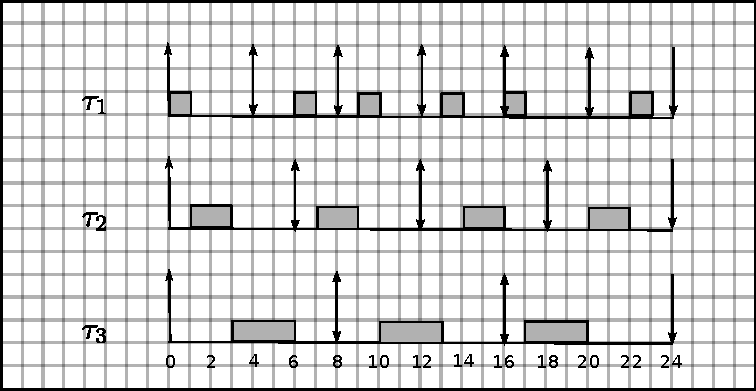
\includegraphics[width=\columnwidth]{images/edf_example}
    \caption{An EDF schedulation example.}
    \label{fig:edf_example}
\end{figure}

Last thing to say is about schedulability bound with EDF:
\begin{itemize}
\item {\bf Theorem}~\cite{LiuL1973}: given a task set of periodic or
  sporadic tasks, with relative deadlines equal to periods, the task
  set is schedulable by EDF if and only if
$$
U = \sum_{i=1}^N \frac{C_{i}}{T_{i}} \leq 1.
$$ 
\item {\bf Corollary}: EDF is an \emph{optimal algorithm} on
  preemptive uniprocessor systems, in the sense that if a task set is
  schedulable, it is schedulable by EDF (you can reach a CPU
  utilization factor of 100\%).
\end{itemize}
We could ensure the schedulability of the task set in
fig.~\ref{fig:edf_example} simply considering that $U = \frac{23}{24}
\leq 1$.

\subsection{Constant Bandwidth Server\label{sec:EDFCBS_CBS}}

In Section~\ref{sec:EDFCBS_EDF} we have considered homogeneous task
set only (periodic or aperiodic). Here we have to cope with scheduling
a task set composed by periodic and aperiodic tasks as well. Periodic
tasks are generally considered of a hard type, whereas aperiodic tasks
may be hard, soft or even non real-time, depending on the application.

Using a periodic task (that is: a \emph{server}), dedicated to serve
aperiodic requests, is possible to have a good average response time
of aperiodic tasks. As every periodic task, a server is characterized
by a period $T_{s}$ and a computing time $C_{s}$, called server
\emph{budget}. A server task is scheduled with the same algorithm used
for periodic tasks, and, when activated, serves the hanging
aperiodic requests (not going beyond its $C_{s}$).

The Constant Bandwidth Server (CBS)~\cite{abeniButtazzo98,
  abeniButtazzo04} is a service mechanism of aperiodic requests on a
dynamic context (periodic tasks are scheduled with EDF) and can be
defined as follows:
\begin{itemize}
\item A CBS is characterized by an ordered pair ($Q_{s}$, $T_{s}$)
  where $Q_{s}$ is the maximum budget and $T_{s}$ is the period of the
  server. The ratio $U_{s} = Q_{s}/T_{s}$ is denoted as the server
  bandwidth.
\item The server manages two internal variables that define its state:
  $c_{s}$ is the current budget at time $t$ (zero-initialized) and
  $d_{s}$ is the current deadline assigned by the server to a request
  (zero-initialized).
\item If a new request arrives while the current request is still
  active, the former is queued in a server queue (managed with an
  arbitrary discipline, for example FIFO).
\item If a new request arrives at instant $t$, when the server is
  idle, you see if you can recycle current budget and deadline of the
  server. If it is $c_{s} \leq (t - d_{s})U_{s}$, then we can schedule
  the request with the current server values, else we have to
  replenish the budget with the maximum value ($c_{s} = Q_{s}$) and
  calculate the deadline as $d_{s} = t + T_{s}$.
\item When a request is completed, the server takes the next (if it
  exists) from the internal queue and schedule it with the current
  budget and deadline.
\item When the budget is exhausted ($c_{s} = 0$), it is recharged at
  the maximum value ($c_{s} = Q_{s}$) and the current deadline is
  postponed of a period ($d_{s} = d_{s} + T_{s}$).
\end{itemize}
The basic idead behind the CBS algorithm is that when a new request
arrives it has a deadline assigned, which is calculated using the
server bandwidth, and then inserted in the EDF ready queue. At the
moment an aperiodic task tries to execute more than the assigned
server bandwidth, its deadline gets postponed, so that its EDF
priority is lowered and other tasks can preempt it.

\subsection{EDF scheduling on SMP systems\label{EDF_SMP}}
In this thesis we will consider the problem of scheduling soft
real-time tasks on a Symmetric Multi Processor (\emph{SMP}) platform,
made up by \emph{M} identical processors (or cores) with constant
speed.

On a multi-core platform, there are three different approaches to
schedule a task set:
\begin{description}
\item[\emph{partitioned}-EDF] tasks are statically assigned to
  processors and those on each processor are scheduled on an EDF
  basis. Tasks are so pinned to a specific runqueue without the
  possibility of migrate between those. Therefore, in an \emph{M}
  processor system we have \emph{M} task sets independently
  scheduled. The main advantage of this approach is its simplicity, as
  a multiprocessor scheduling problem is reduced to \emph{M}
  uniprocessor ones. Furthermore, tasks experience no overhead, since
  there arent't migrations. On the contrary, drawbacks of P-EDF are
  the complexity to find an optimal assignment of tasks to processors
  (which is NP-hard) and the impossibility to schedule some particular
  task sets that are schedulable only if task sets are not
  partitioned~\cite{HOS}.
\item[\emph{global}-EDF] jobs are inserted in a global
  deadline-ordered ready queue, and on a instant by instant basis the
  available processors are allocated to the nearest deadline jobs in
  the ready queue.
\item[\emph{hybrid}-EDF] tasks are statically assigned to fixed-size
  clusters, much as tasks are assigned to processors in P-EDF. The
  G-EDF algorithm is then used to schedule the tasks on each cluster,
  as if each cluster be constituted by an independent system for
  scheduling purposes.
\end{description}
No variant of EDF is optimal, so deadline misses can occur under each
EDF variant in a feasible systems\footnote{Systems with total
  utilization at most the number of processors}.  It has been shown,
however, that deadline tardiness under G-EDF is bounded in systems,
which, as we said, is sufficient for many soft real-time applications
~\cite{devi_tardiness, valente_lateness}.

Under the H-GDF approach, deadline tardiness is bounded for each
cluster as long as the total utilization of the tasks assigned to each
cluster is at most the number of cores per cluster.

\section{The
  SCHED\_DEADLINE scheduling class \label{sec:schedDead}}

\texttt{SCHED\_DEADLINE}~\cite{SCHEDDEAD} is a scheduling policy
(made by Dario Faggioli and Michael Trimarchi), implemented inside its
own scheduling class, aiming at introducing deadline scheduling for
Linux tasks.  It is being developed by Evidence
S.r.l.~\footnote{\url{http://www.evidence.eu.com}} in the context of
the EU-Funded project
ACTORS~\footnote{\url{http://www.actors-project.eu/}}.

The need of an EDF scheduler in Linux has been already highlighted in
the \texttt{Documentation/scheduler/sched-rt-group.txt} file, which
says: \emph{``The next project will be SCHED\_EDF (Earliest Deadline
  First scheduling) to bring full deadline scheduling to the linux
  kernel''}. Developers have actually chosen the name
\texttt{SCHED\_DEADLINE} instead of \texttt{SCHED\_EDF} because EDF is
not the only deadline algorithm and, in the future, it may be
desiderable to switch to a different algorithm without forcing
applications to change which scheduling class they request.

The partners involved in this project (which include Ericsson
Research, Evidence S.r.l., AKAtech) strongly believe that a
general-purpose operating system like Linux should provide a standard
real-time scheduling policy still allowing to schedule non real-time
tasks in the usual way.

The existing scheduling classes (i.e., \texttt{SCHED\_FAIR} and
\texttt{SCHED\_RT}, see fig.~\ref{fig:modular_scheduler}) perform very well in
their own domain of application. However,
\begin{itemize}
\item they cannot provide the guarantees a time-sensitive application
  may require. The point has been analyzed for \texttt{SCHED\_FIFO}
  and \texttt{SCHED\_RR} policies (refer to
  sec.~\ref{sec:StateArt_FIFO}); using \texttt{SCHED\_FAIR} no concept
  of timing constraint can be associated to tasks as well.
\item The latency experienced by a task (i.e., the time between two
  consecutive executions of a task) is not deterministic and cannot be
  bound, since it highly depends on the number of tasks running in the
  system at that time.
\end{itemize}
It has to be emphasized the fact that these issues are particularly
critical when running time-sensitive or control applications. Without
a real-time scheduler, in fact, it is not possible to make any
feasibility study of the system under development, and developers
cannot be sure that the timing requirements will be met under
\emph{any circumstance}. This prevents the usage of Linux in
industrial context.

\subsection{Main Features}\label{sec:schedDead_main}

\texttt{SCHED\_DEADLINE}~\footnote{The new \texttt{kernel/sched/dl.c}
  file contains the scheduling policy core.} implements the Earliest
Deadline First algorithm and uses the Constant Bandwidth Server to
provide \emph{bandwidth isolation}~\footnote{Different tasks cannot
  interfere with each other, i.e., CBS ensures each task to run for at
  most its runtime every (relative) deadline length time interval.}
among tasks. The scheduling policy does not make any restrictive
assumption about the characteristics of tasks: it can handle periodic,
sporadic or aperiodic tasks.

This new scheduling class has been developed from scratch, without
starting from any existing project, taking advantage of the modularity
currently offered by the Linux scheduler, so as not to be too
invasive. The implementation is aligned with the current (at the time
of writing) mainstream kernel, and it will be kept lined up with
future kernel versions.

\texttt{SCHED\_DEADLINE} relies on standard Linux mechanisms (e.g.,
control groups) to natively support multicore platforms and to provide
hierarchical scheduling through a standard API.

\subsection{Interaction with Existing Policies}\label{sec:schedDead_interaction}

The addition of the \texttt{SCHED\_DEADLINE} scheduling class to the
Linux kernel does not change the behavior of the existing scheduling
policies, neither best-effort and real-time ones. However, given the
current Linux scheduler architecture, there is some interaction
between scheduling classes. In fact, since each class is asked to
provide a runnable task in the order they are chained in a linked
list, ``lower'' classes actually run in the idle time of ``upper''
classes. Where to put the new scheduling class is a key point to
obtain the right behavior. Developers chose to place it above the
existing real-time and normal scheduling classes, so that deadline
scheduling can run at the highest priority, otherwise it cannot ensure
that the deadlines will be met.  

Figure~\ref{fig:new_modular_scheduler} shows the Linux scheduling
framework with \texttt{SCHED\_DEADLINE} added.

\begin{figure}[htbp]
    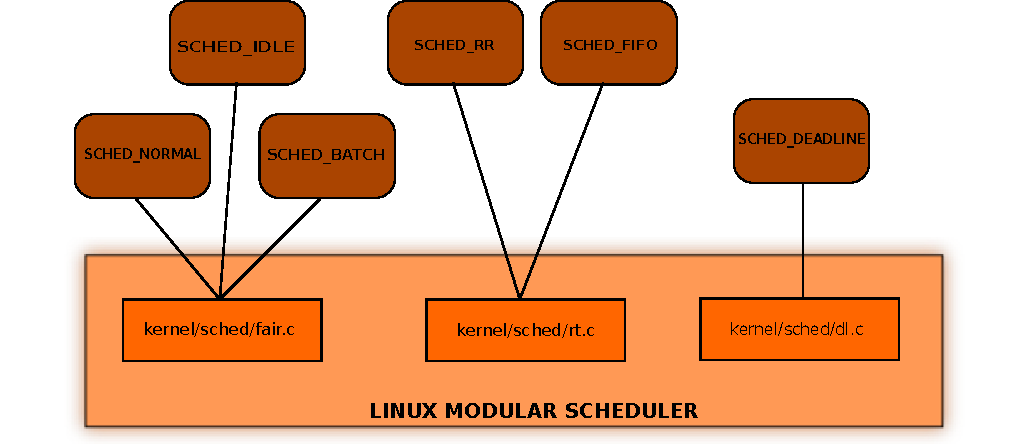
\includegraphics[width=\columnwidth]{images/new_modular_scheduler}
    \caption{The Linux modular scheduling framework with
\texttt{SCHED\_DEADLINE}.}
    \label{fig:new_modular_scheduler}
\end{figure}

\subsection{Current Multiprocessor Scheduling Support}\label{sec:schedDead_multiproc}

As we have seen in Section~\ref{sec:LinuxSched_runqueue}, in Linux
each CPU has its own ready queue, so the way Linux deals with
multiprocessor scheduling is often called \emph{distributed
  runqueue}. Tasks can, if wanted or needed, migrate between the
different queues. It is possible to pin some task on some processor,
or set of processors, setting the so called \emph{scheduling
  affinity} as well.

SCHED\_DEADLINE developers has initially chose to implement the P-EDF
solution, where no dynamic processes migration can take place, unless
we change the task
affinity.

Recently, Juri Lelli, the current mantainer of SCHED\_DEADLINE
project, has extended its implementation to allow a G-EDF and a H-EDF
schedulation schemes.  At the time of writing, in SCHED\_DEADLINE
newer version, we found not only the same distributed runqueue
approach that all other scheduling classes follow, but also the push
and pull algorithms to balance the load over all CPUs in the system.
Obviously, here the migrations are done comparing the tasks deadline.\\
The goal of this design is to approximate as much as possible the
G-EDF rule: ``on an \emph{M} CPUs system, the \emph{M} earliest
deadline ready tasks run on the CPUs''. We use the term approximate
because it's clear that there may be some intervals in which the above
rule may be violated: in fact, scheduler can migrate tasks only when
they are woken up or when their relative deadline changes, in a
similar manner as we have seen in \ref{sec:MULTICORERT_PUSH_PULL} for
\texttt{SCHED\_RT} scheduling class tasks. In other words, the
scheduler uses only local informations to impose a schedule, while
occasionally relying on the push and pull mechanisms to
achieve a global balancing.

Compared to a global scheduling policy with a single system-wide
runqueue, this solution has the advantage of a better scalability as
the number of underlying cores increases. In fact, we have to keep in
mind that, on a \emph{M} processors SMP system, we can have up to
\emph{M} scheduler instances executing at the same time,
that compete to acquire the lock on the single runqueue.

Now, let us briefly discuss the data structures and the algorithms
behind the \texttt{SCHED\_DEADLINE} support to multi-core
environments.

The concept of root domain is used here as in \texttt{SCHED\_RT}, but
the \texttt{struct root\_domain} is extended to manage the deadline
tasks, so we can find the following additional fields:

\begin{lstlisting}[language=C, caption={\texttt{struct root\_domain extended}},
			label={lst:struct_root_domain_ext}]

struct root_domain {
	<same fields as above>
	...
	cpumask_var_t dlo_mask;
	atomic_t dlo_count;
	...
	struct cpudl cpudl;
};

\end{lstlisting}

The field \texttt{dlo\_mask} shows which CPUs are overloaded and
\texttt{dlo\_count} keeps count of those. The remaining field,
\texttt{struct cpudl}, is fundamental to speed up the push
mechanism. In the current implementation, that data structure is a
max-heap that keeps the deadline of the earliest deadline task in all
the runqueue.

As we will see in the remaining part of this document, the main goal
of this thesis it to design and develop more efficient data structures
to speed up the migration algorithms.

To implement the tasks migration mechanism, \texttt{SCHED\_DEADLINE}
also uses some particular fields on his runqueue structure, as we can
see in Listing~\ref{lst:struct_dl_rq}.

\begin{lstlisting}[language=C, caption={\texttt{struct dl\_rq}},
                        label={lst:struct_dl_rq}]

struct dl_rq {
	struct rb_root;
	struct rb_node *rb_leftmost;
	unsigned long dl_nr_running;

#ifdef CONFIG_SMP
	struct {
		u64 curr;
		u64 next;
	} earliest_dl;
	
	unsigned long dl_nr_migratory;
	unsigned long dl_nr_total;
	int overladed;

	struct rb_root pushable_dl_tasks_root;
	struct rb_node *pushable_dl_tasks_leftmost;
#endif
	...
};

\end{lstlisting}

The \texttt{struct dl\_rq} is the place where we store task accounting
informations to manage overloading and migrations. Among these the most
important fields are:
\begin{description}
\item[\texttt{struct earliest\_dl}] a cache for the two earliest deadline
task enqueued in the runqueue, to speed up push and pull decisions.
\item[\texttt{dl\_nr\_migratory}] the number of deadline tasks that can
migrate.
\item[\texttt{dl\_nr\_total}] total number of deadline tasks queued.
\item[\texttt{pushable\_dl\_tasks\_root}] the root of a red-black tree
where pushable deadline tasks are enqueued.
\item[\texttt{pushable\_tasks\_leftmost}] pointer to the earliest deadline
pushable task.
\end{description}

\subsection{\texttt{SCHED\_DEADLINE} Push implementation\label{sec:push_dl_impl}}
Now, let us discuss in great detail the push algorithm implemented in \texttt{SCHED\_DEADLINE}
scheduling class. In Listing~\ref{lst:push_dl} we can see the main push mechanism 
function: \texttt{push\_dl\_task}.

\begin{lstlisting}[language=C, caption={\texttt{\emph{Push} function}},
				label={lst:push_dl}]

static int push_dl_task {
	struct task_struct *next_task;
	struct rq *later_rq;
	
	if (!rq->dl.overloaded)
		return 0;

	next_task = pick_next_pushable_dl_task(rq);
	if (!next_task)
		return 0;
	
retry:
	if (unlikely(next_task == rq->curr)) {
		WARN_ON(1);
		return 0;
	}

	/*
	 * If next_task preempts rq->curr, and rq->curr
	 * can move away, it makes sense to just reschedule
	 * without going further in pushing next_task.
	 */
	if (dl_task(rq->curr) &&
		dl_time_before(next_task->dl.deadline, rq->curr->dl.deadline) &&
		rq->curr->dl.nr_cpus_allowed > 1) {
		resched_task(rq->curr);
		return 0;
	}

	/* We might release rq lock */
	get_task_struct(next_task);

	/* Will lock the rq it'll find */
	later_rq = find_lock_later_rq(next_task, rq);
	if (!later_rq) {
		struct task_struct *task;

		/*
		 * We must check all this again, since
		 * find_lock_later_rq releases rq->lock and it is
		 * then possible that next_task has migrated.
		 */
		task = pick_next_pushable_dl_task(rq);
		if (task_cpu(next_task) == rq->cpu && task == next_task) {
			/*
			 * The task is still there. We don't try
			 * again, some other cpu will pull it when ready.
			 */
			dequeue_pushable_dl_task(rq, next_task);
			goto out;
		}

		if (!task)
			/* No more tasks */
			goto out;

		put_task_struct(next_task);
		next_task = task;
		goto retry;
	}
	
	deactivate_task(rq, next_task, 0);
	set_task_cpu(next_task, later_rq->cpu);
	activate_task(later_rq, next_task, 0);

	resched_task(later_rq, next_task, 0);

	double_unlock_balance(rq, later_rq);

out:
	put_task_struct(next_task);

	return 1;
};

\end{lstlisting}

The \emph{push} function first checks the overloaded flag to see if
there are deadline tasks to push away, then pick from the pushable
rbtree the task to try to push next. At this time,
\texttt{find\_lock\_later\_rq} find and lock a runqueue where the task
can immediately run, that is, the pushable task will preempt the task
currently executing on the target runqueue. If such a runqueue is
found then the actual migration is accomplished, otherwise the
function just retries or exits.

The \texttt{find\_lock\_later\_rq} code is presented in
Listing~\ref{lst:pick_next_pushable_dl_task}.

\begin{lstlisting}[language=C, caption={\texttt{\emph{pick\_next\_pushable\_dl\_task} function}},
				label={lst:pick_next_pushable_dl_task}]

static struct rq *find_lock_later_rq(struct task_struct *task, struct rq *rq)
{
	struct rq *later_rq = NULL;
	int tries;
	int cpu;

	for(tries = 0; tries < DL_MAX_TRIES; tries++) {
		cpu = find_later_rq(task);

		if ((cpu == -1) || (cpu == rq->cpu))
			break;

		later_rq = cpu_rq(cpu);

		/* Retry if something changed. */
		if (double_lock_balance(rq, later_rq)) {
			if (unlikely(task_rq(task) != rq ||
				!cpumask_test_cpu(later_rq->cpu,
					&task->cpus_allowed) ||
				task_running(rq, task) ||
				!task->on_rq)) {
				double_unlock_balance(rq, later_rq);
				later_rq = NULL;
				break;
			}
		}

		/*
		 * If the runqueue we found has no -deadline task, or
		 * its earliest one has a later deadline than our
		 * task, the rq is a good one.
		 */
		if(!later_rq->dl.dl_nr_running ||
			dl_time_before(task->dl.deadline,
				later_rq->dl.earliest_dl.curr))
			break;

		/* Otherwise we try again */
		double_unlock_balance(rq, later_rq);
		later_rq = NULL;
	}
	
	return later_rq;
} 

\end{lstlisting}

This function tries up to \texttt{DL\_MAX\_TRIES} (that is, three times in the
current implementation) times to find a suitable
runqueue to push the task away. It only acquires a double lock, one on the 
source and the other on the destination runqueues if it succeeds in its work.
A check is performed immediately after that the locks are acquired to see if
a parallel scheduling operation makes the target runqueue no more eligible to
immediately run the task to migrate. 
The very core of all mechanism is inside the \texttt{find\_later\_rq} function.
Here we show only the relevant part:

\begin{lstlisting}[language=C, caption={\texttt{find\_later\_rq} function},
				label={lst:find_later_rq}]

static int find_later_rq(struct task_struct *task)
{
	struct sched_domain *sd;
	struct cpumask *later_mask = __get_cpu_var(local_cpu_mask_dl);
	int this_cpu = smp_processor_id();
	int best_cpu, cpu = task_cpu(task);

	/* Make sure the mask is initialized first */
	if (unlikely(!later_mask))
		return -1;

	if (task->dl.nr_cpus_allowed == 1)
		return -1;

	best_cpu = cpudl_find(&task_rq(task)->rd->cpudl,
			task_rq(task)->rd->dlo_mask,
			task, later_mask);
	if (best_cpu == -1)
		return -1;

	...

	return best_cpu;
}

\end{lstlisting}

\subsection{Max-heap \texttt{cpudl} data structure for push operation\label{sec:max_heap_cpudl}}

As we have seen, the function \texttt{find\_later\_rq} relies on the
\texttt{cpudl} data structure to efficiently find a target runqueue
(that is, a target CPU) where to push the task.

In the current \texttt{SCHED\_DEADLINE} implementation the
\texttt{cpudl} data structure is a max-heap that stores the deadline
value of the tasks currently executing on a CPU. We can see an example
of such a structure in Figure~\vref{fig:cpudl_push} where a 4-CPUs
system is represented.  In the above Figure the \texttt{cpudl} data
structure is simply represented as an ordered queue, since we will see
that many possible solutions are available for the implementation of
such a structure.

The \texttt{cpudl} data structure is managed through a simple API made
up of two function, as we can see in Listing~\ref{lst:cpudl_interf}.

\begin{lstlisting}[language=C, caption={\texttt{cpudl} API},
				label={lst:cpudl_interf}]

int cpudl_find(struct cpudl *cp, struct cpumask *dlo_mask,
		struct task_struct *p, struct cpumask *later_mask);
void cpudl_set(struct cpudl *cp, int cpu, u64 dl, int is_valid);

\end{lstlisting}

The \emph{find} operation is called when a scheduler instance, running on a CPU,
has to migrate a task and needs to know where it can push one.

The \emph{set} operation is called when a scheduler instance, running
on a CPU, has to update the \texttt{cpudl} data structure to reflect a
change in the underlying runqueue status.

To implement a scheduling policy as close as possible to \emph{G-EDF},
the \emph{cpudl} data structure keeps also track of the free CPUs
(that is, a CPU with no deadline tasks enqueued in its runqueue). When
a CPU needs to know where to push a task, \texttt{cpudl\_find} first
looks into a proper CPU bitmask where all free CPUs has an associated
cleared bit. If it is possible to find at least one free CPU, we don't
have to search in the
max-heap and we can immediately return the CPU index founded.

Now, let us focus on the \texttt{cpudl\_find} and \texttt{cpudl\_set}
parameters. Regarding the former operation, we have the following
parameters:

\begin{description}
\item[\texttt{cp}] same as above.
\item[\texttt{dlo\_mask}] not used in current version.
\item[\texttt{p}] a pointer to the task to migrate. We use this pointer
to read the CPU affinity of the task in its \emph{task\_struct}. In this
way, \texttt{cpudl\_find} can always returns an eligilble CPU index where
task \texttt{p} is allowed to run.
\item[\texttt{later\_mask}] a pointer to a CPU bitmask where 
\texttt{cpudl\_find} can set all bits related to CPUs eligible for the migration.
In particular, this mask is used when there are more than one free CPUs and
\texttt{cpudl\_find} lets the caller choose which CPU is best.
\end{description}

Regarding the latter one, we have to specify the following parameters:

\begin{description}
\item[\texttt{cp}] a pointer to the instance of the \texttt{cpudl} data
structure. In fact, there are as many different instances of \texttt{cpudl} data
structures as the number of root domains.
\item[\texttt{cpu}] the index of the CPU that is calling the function.
\item[\texttt{dl}] the new deadline value of the currently running task on
\texttt{cpu}.
\item[\texttt{is\_valid}] a flag to indicate if there is at least one
\end{description}

deadline task enqueued in the runqueue.

\begin{figure}[htbp]
    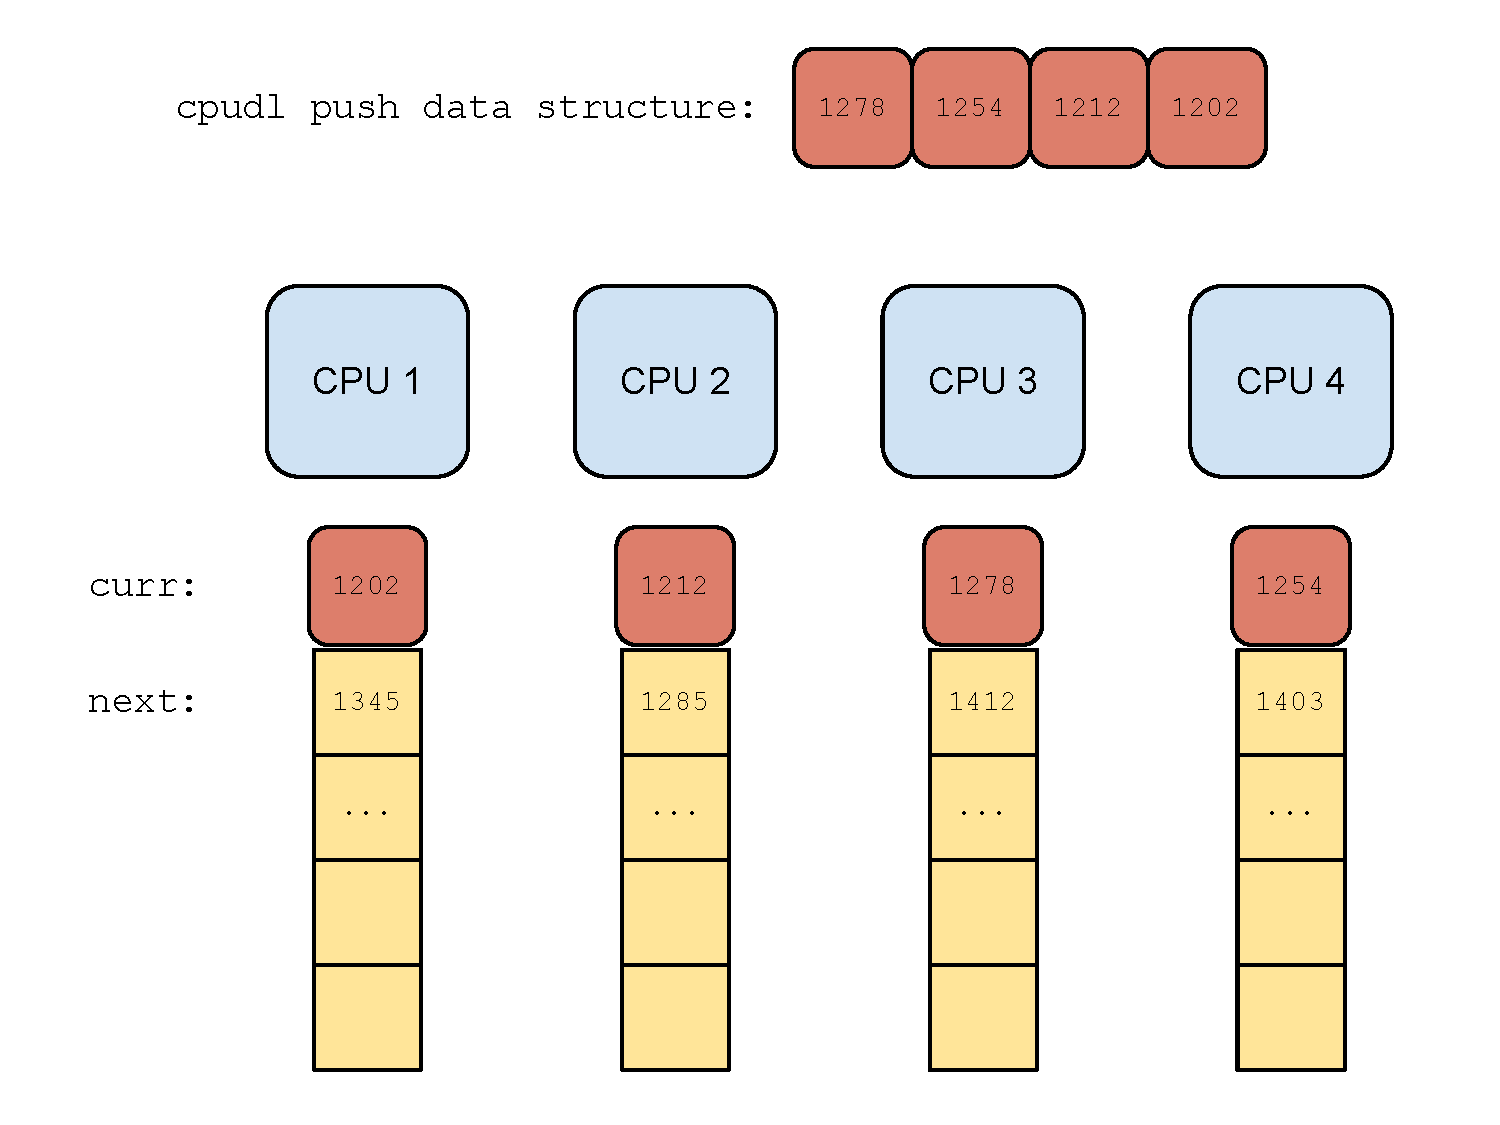
\includegraphics[width=\columnwidth]{images/Push_cpudl}
    \caption{\texttt{cpudl} structure for \emph{push} operation.}
    \label{fig:cpudl_push}
\end{figure}

\subsection{\texttt{SCHED\_DEADLINE} Pull implementation\label{sec:pull_dl_impl}}

The \emph{pull} function checks all the root domain's overloaded
runqueues to see if there is a task that the calling runqueue can take
in order to run it immediately.  If found, this function performs a
migration, otherwise it continues or just exits if there are no more
runqueue to consider. So, we can state that the main goal of both push
and pull operations is to perform a preemption in the target runqueue.

The pull operation in implemented in the \texttt{pull\_dl\_task}
function, presented in Listing~\ref{lst:pull_dl_task}. For brevity's
sake we remove all the comments from the code.

\begin{lstlisting}[language=C, caption={\texttt{\emph{pull\_dl\_task} function}},
				label={lst:pull_dl_task}]

static int pull_dl_task(struct rq *this_rq)
{
	int this_cpu = this_rq->cpu, ret = 0, cpu;
	struct task_struct *p;
	struct rq *src_rq;
	u64 dmin = LONG_MAX;

	if (likely(!dl_overloaded(this_rq)))
		return 0;

	for_each_cpu(cpu, this_rq->rd->dlo_mask) {
		if (this_cpu == cpu)
			continue;

		src_rq = cpu_rq(cpu);
		
		if (this_rq->dl.dl_nr_running &&
			dl_time_before(this_rq->dl.earliest_dl.curr,
					src_rq->dl.earliest_dl.next))
			continue;
		
		double_lock_balance(this_rq, src_rq);
		
		if (src_rq->dl.dl_nr_running <= 1)
			goto skip;

		p = pick_next_earliest_dl_task(src_rq, this_cpu);

		if (p && dl_time_before(p->dl.deadline, dmin) &&
			(!this_rq->dl.dl_nr_running ||
			dl_time_before(p->dl.deadline,
					this_rq->dl.earliest_dl.curr))) {
			WARN_ON(p == src_rq->curr);
			WARN_ON(!p->on_rq);

			if (dl_time_before(p->dl.deadline,
					src_rq->curr->dl.deadline))
				goto skip;

			ret = 1;

			deactivate_task(src_rq, p, 0);
			set_task_cpu(p, this_cpu);
			activate_task(this_rq, p, 0);
			dmin = p->dl.deadline;
		}
skip:
		double_unlock_balance(this_rq, src_rq);
	}

	return ret;
}

\end{lstlisting}

The key difference between the \emph{pull} operation and the
\emph{push} function, is that inside pull we have to check every
single runqueue in order to find tasks to pull. In other words, in the
current implementation, there isn't available an analogous data
structure like the \texttt{cpudl} one for the \emph{push} operation.
On a large SMP system, with a considerable number of cores, this can
lead to an unsustainable latency to perform the \emph{pull} operation.

We will see in Chapter~\ref{chap:data_struct_dev} how we have addressed this problem.

\subsection{Task Scheduling}\label{sec:schedDead_scheduling}
As mentioned earlier, \texttt{SCHED\_DEADLINE} does not make any
restrictive assumption on the characteristics of its tasks, thus it
can handle:

\begin{itemize}
\item periodic tasks, typical in real-time and control applications;
\item aperiodic tasks;
\item sporadic tasks (i.e., aperiodic tasks with a \emph{minimum interarrival
time} (\emph{MIT}) between releases), typical in soft real-time and multimedia
applications;
\end{itemize}

A key feature of task scheduling in this scheduling class is that
\emph{temporal isolation} is ensured (while this feature is not
available in \texttt{SCHED\_RT} scheduling class, as we seen in
Section~\ref{sec:StateArt_FIFO}).  This means that the temporal
behavior of each task (i.e., its ability to meet its deadlines) is not
affected by the behavior of any other task in the system. So, even if
a task misbehaves, it is not able to exploit larger execution time
than it has been allocated to it and monopolize the processor.

Each task is assigned a \emph{budget} (\texttt{sched\_runtime} and a
\emph{period}, considered equal to its \emph{deadline} (\texttt{sched\_period}).
The task is guaranteed to execute for an amount of time equal to
\texttt{sched\_runtime} every \texttt{sched\_period} (task \emph{utilization} or
\emph{bandwidth}). When a task tries to execute more than its \emph{budget} it
is slowed down, by stopping it until the time instant of its next deadline.
When, at that time, it is made runnable again, its budget is refilled and a new
deadline computed for him. This is how the CBS algorithm works, in its
hard-reservation configuration.

This way of working goes well for both aperiodic and sporadic tasks, but it
imposes some overhead to ``standard'' periodic tasks. Therefore, the developers
have made it possible for periodic tasks to specify, before going to sleep
waiting for the next activation, the end of the current instance. This avoid
them (if they behave well) being disturbed by the CBS.

\subsection{Usage and Tasks API}\label{sec:schedDead_API}
\texttt{SCHED\_DEADLINE} users have to specify, before running their real-time
application, the system wide \texttt{SCHED\_DEADLINE} bandwidth. They can do
this echoing the desired values in
\texttt{/proc/sys/kernel/sched\_dl\_}\\
\texttt{period\_us} and
\texttt{/proc/sys/kernel/sched\_dl\_runtime\_us}\\
files. The quantity
$$
\frac{\texttt{sched\_dl\_runtime\_us}}
{\texttt{sched\_dl\_period\_us}}
$$
will be the overall system wide bandwidth \texttt{SCHED\_DEADLINE} tasks are
allowed to use.\\
Otherwise, it is possible to disable \texttt{SCHED\_DEADLINE} bandwidth control echoing
the value -1 to in \texttt{/proc/sys/kernel/sched\_dl\_runtime\_us}.\\
The existing system call \texttt{sched\_setscheduler(\dots)} has not been
extended, because of the binary compatibility issues that modifying its
\texttt{struct sched\_param} parameters would have raised for existing
applications. \\
Therefore, another system call, called \texttt{struct sched\_param2}
\footnote{defined in include/linux/sched.h} has been implemented. 
It allows to assign or modify the scheduling parameters described above 
(i.e., \texttt{sched\_dl\_runtime} and \texttt{sched\_dl\_period})
for tasks running with \texttt{SCHED\_DEADLINE} policy. \\
The \texttt{struct sched\_param2} implementation can be seen in
Listing~\ref{lst:struct_sched_param2}.

\begin{lstlisting}[language=C, caption={\texttt{struct sched\_param2}},
                        label={lst:struct_sched_param2}]
struct sched_param2 {  
    int sched_priority;  
    unsigned int sched_flags;  
    u64 sched_runtime;  
    u64 sched_deadline;  
    u64 sched_period;  
};

\end{lstlisting}

The syscall has the following prototype:

\begin{lstlisting}[language=C, caption={\texttt{sched\_setscheduler2} syscall},
			label={lst:sched_setscheduler2}]

int sched_setscheduler2(struct task_struct *p, int policy,
			const struct sched_param2 *param);

\end{lstlisting}

For the sake of consistency, also 

\begin{lstlisting}[language=C, caption={\texttt{sched\_setparam2} and \texttt{sched\_getparam2} syscalls}]
int sched_setparam2(pid_t pid, struct sched_param2 *param);
int sched_getparam2(pid_t pid, struct sched_param2 *param);
\end{lstlisting}

have been implemented.
